\section{DFT spectral multiplication}
We will now try to show that a there is another way doing filtering with spectral multiplication in frequency domain instead of convolution in time domain. A guiding figure \ref{fig:DFTTeori} is shown below.
We first take convolution of the signal with the filter to represent the time domain filtering. Secondly we take the filter , the data and fft transform them independently, multiply them in the frequency domain and reverse fft them back to time domain.
The plot of time domain for both methods can be seen on figure \ref{fig:dftmethods}
We see a good overlap of the two methods although not an exact fit, we expect this to be a problem wit the way we filter the data and not cutting of the "wings".

\begin{figure}[h]
  \centering
  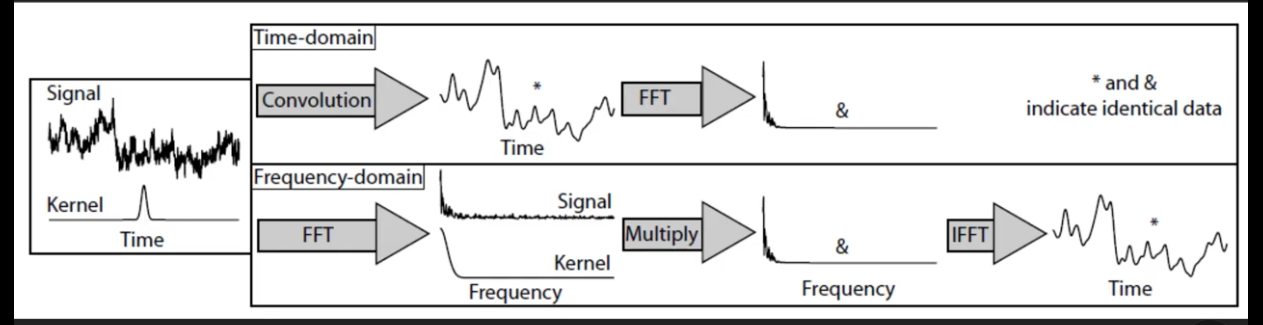
\includegraphics[width=\textwidth]{matlabstuff/covmulti.png}
  \caption{Time domain filtering versus frequency domain}%
  \label{fig:DFTTeori}
\end{figure}


\begin{figure}[h]
  \centering
  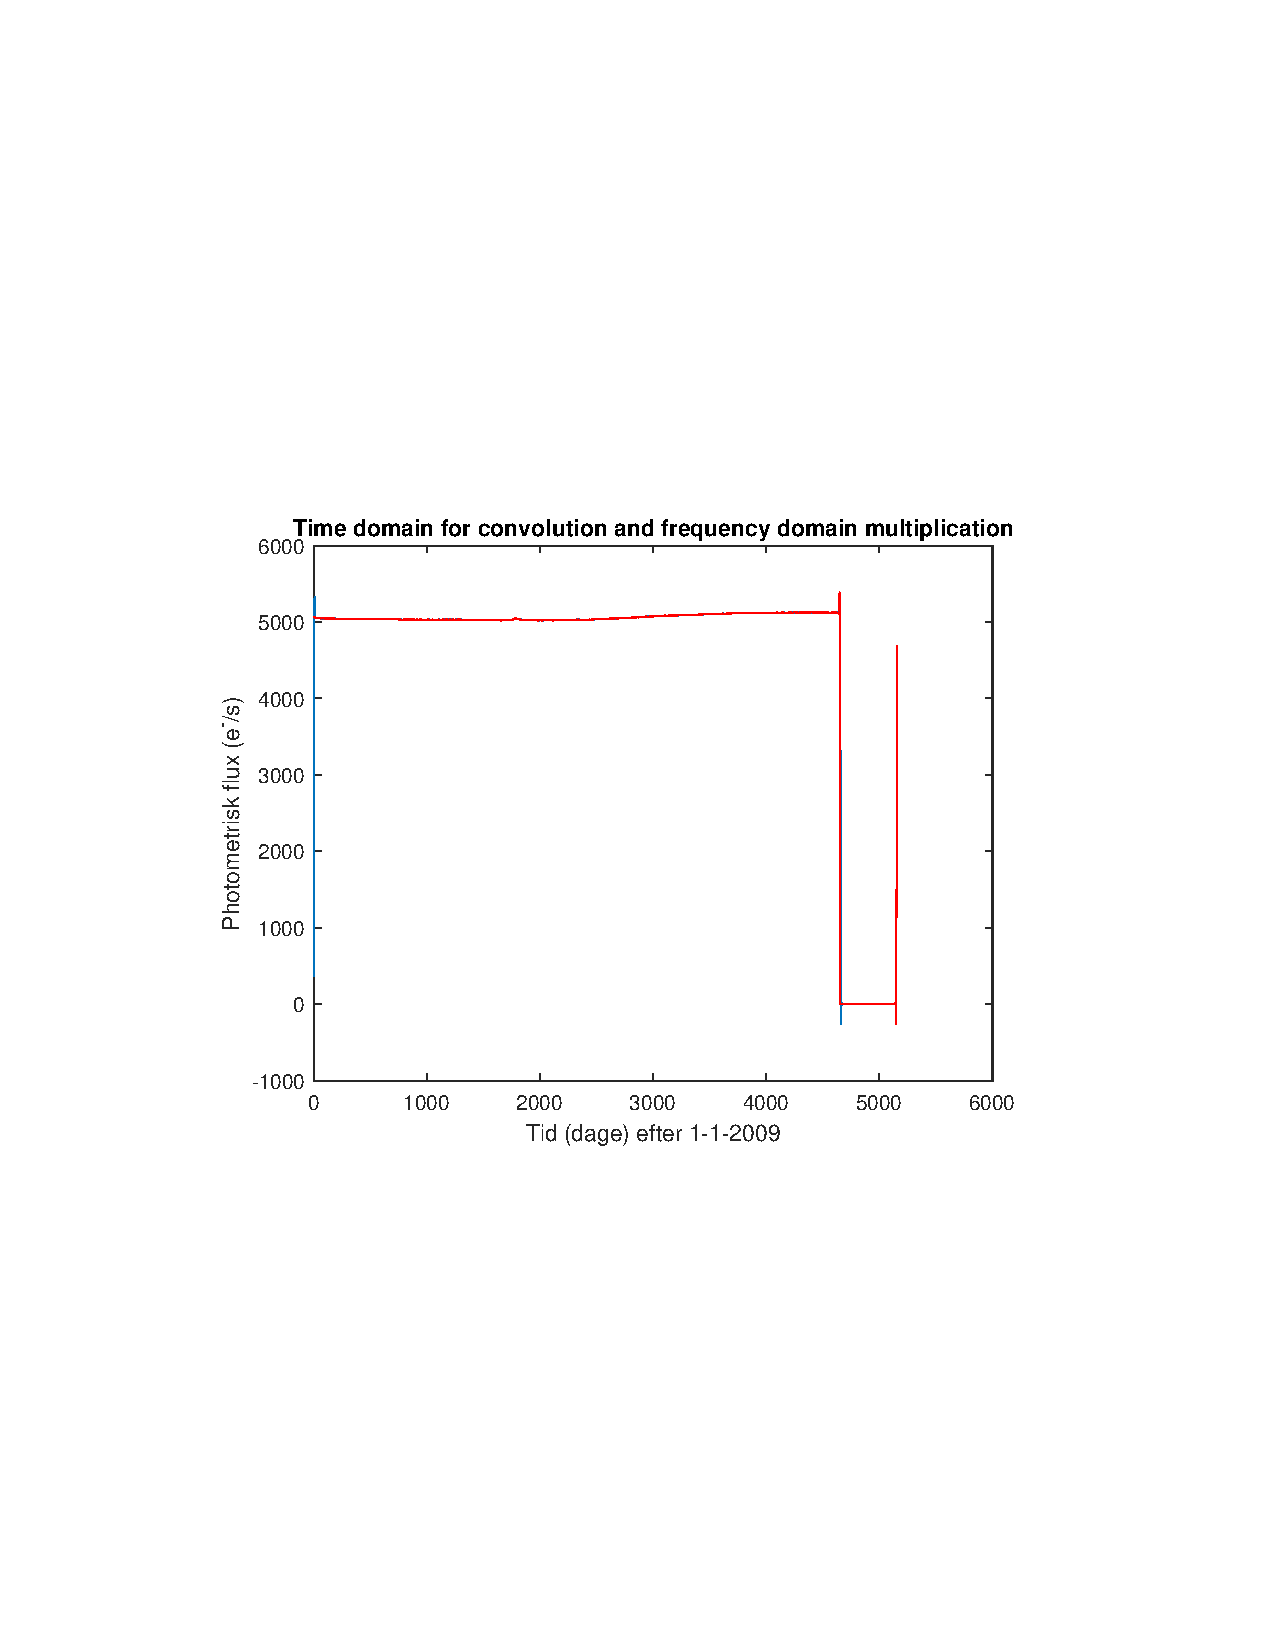
\includegraphics[width=\textwidth]{matlabstuff/dft-methods.pdf}
  \caption{Time domain filter for both methods.}%
  \label{fig:dftmethods}
\end{figure}


\section{STFT of kepler data}

Here we try use Matlab STFT spectrogram function to look for any prevalent frequency change over the observation time. 
We try to find a windows function that will give us more frequency resolution, the data is already very noisy and normal rectangular window will give a lot of articulates that will pollute the spectral plot. We go with blackman. The windows size is a trade-of between time resolution and frequency resolution, we go for something in between and as the number of samples is 4654 we go for 128.    
\\
The spectrogram plot is shown in figure \ref{fig:STFT}. It is very difficult to see any change. This is due to very low data count and slow / very small changes, coupled with a lot of noise. 

\begin{figure}[h]
  \centering
  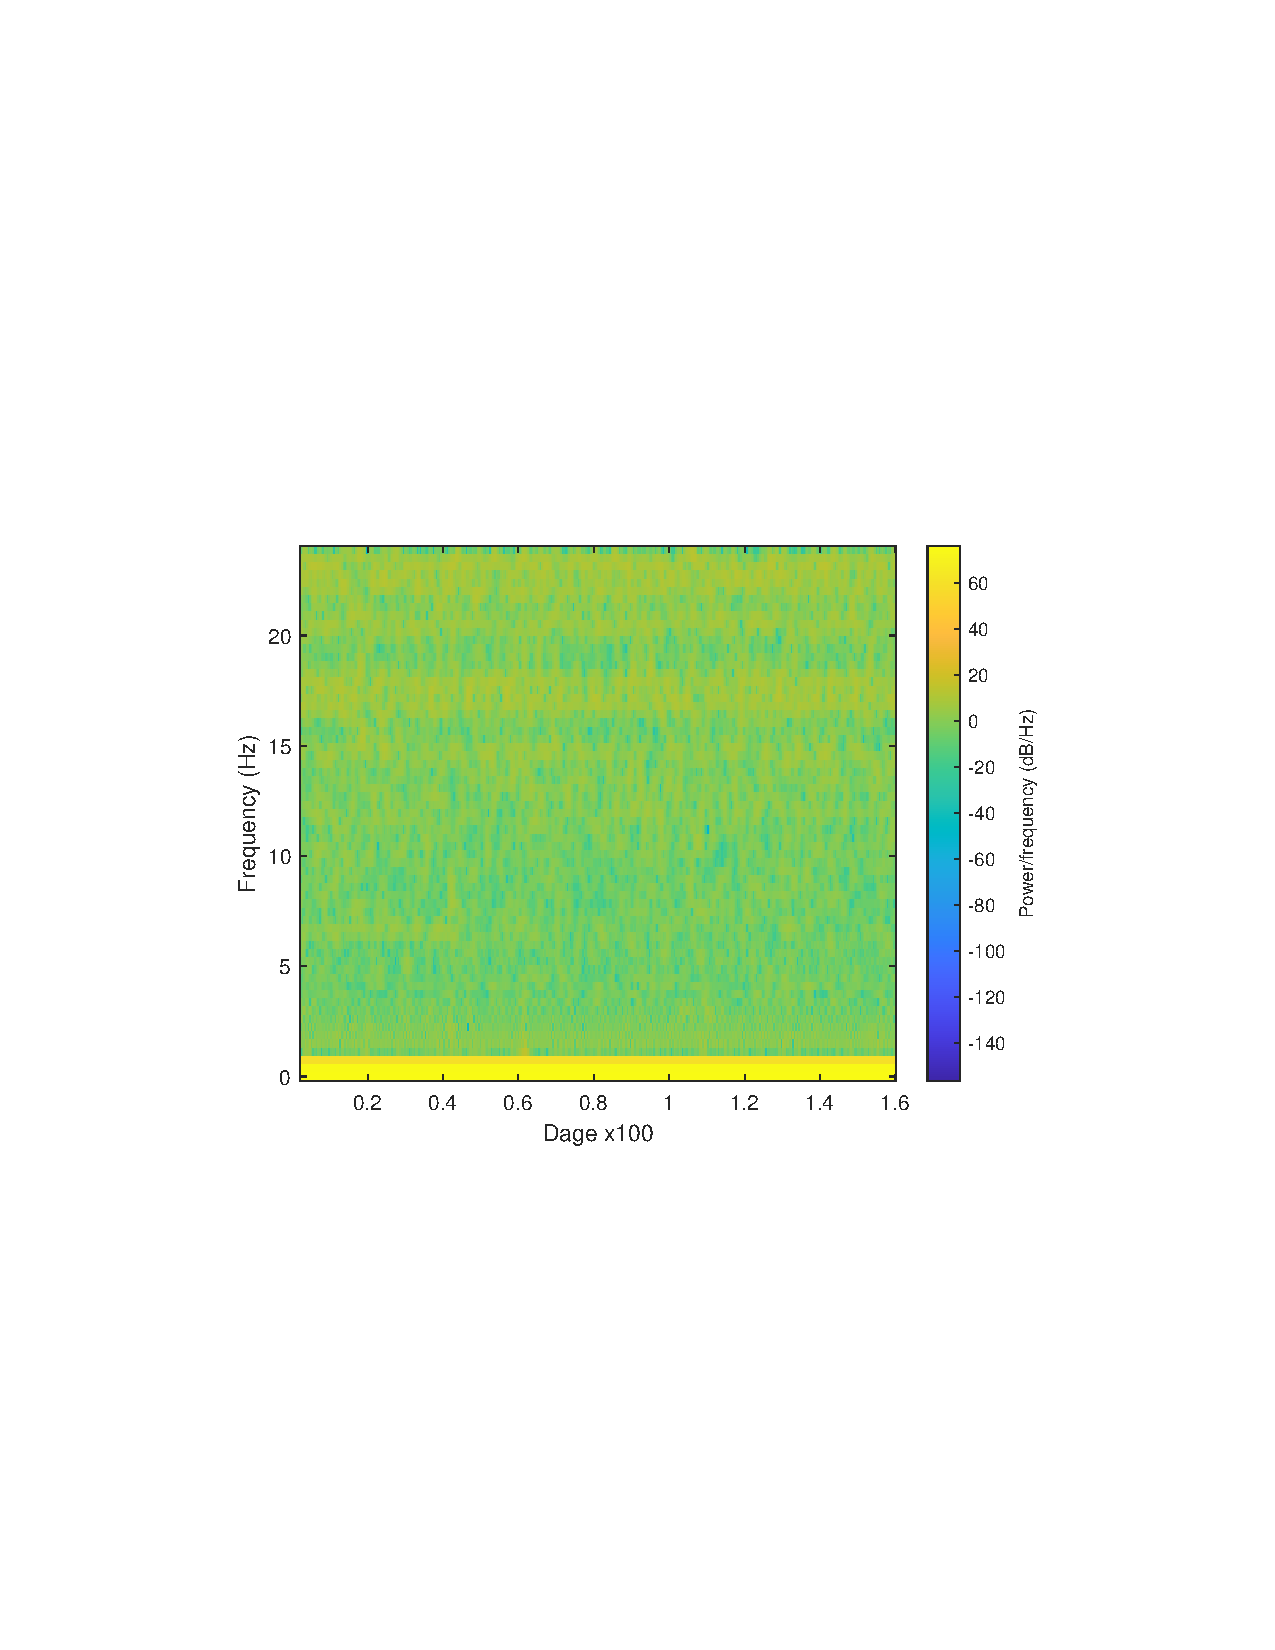
\includegraphics[width=\textwidth]{matlabstuff/STFT.pdf}
  \caption{STFT spectrogram of the kepler data}%
  \label{fig:STFT}
\end{figure}

\begin{figure}[h]
  \centering
  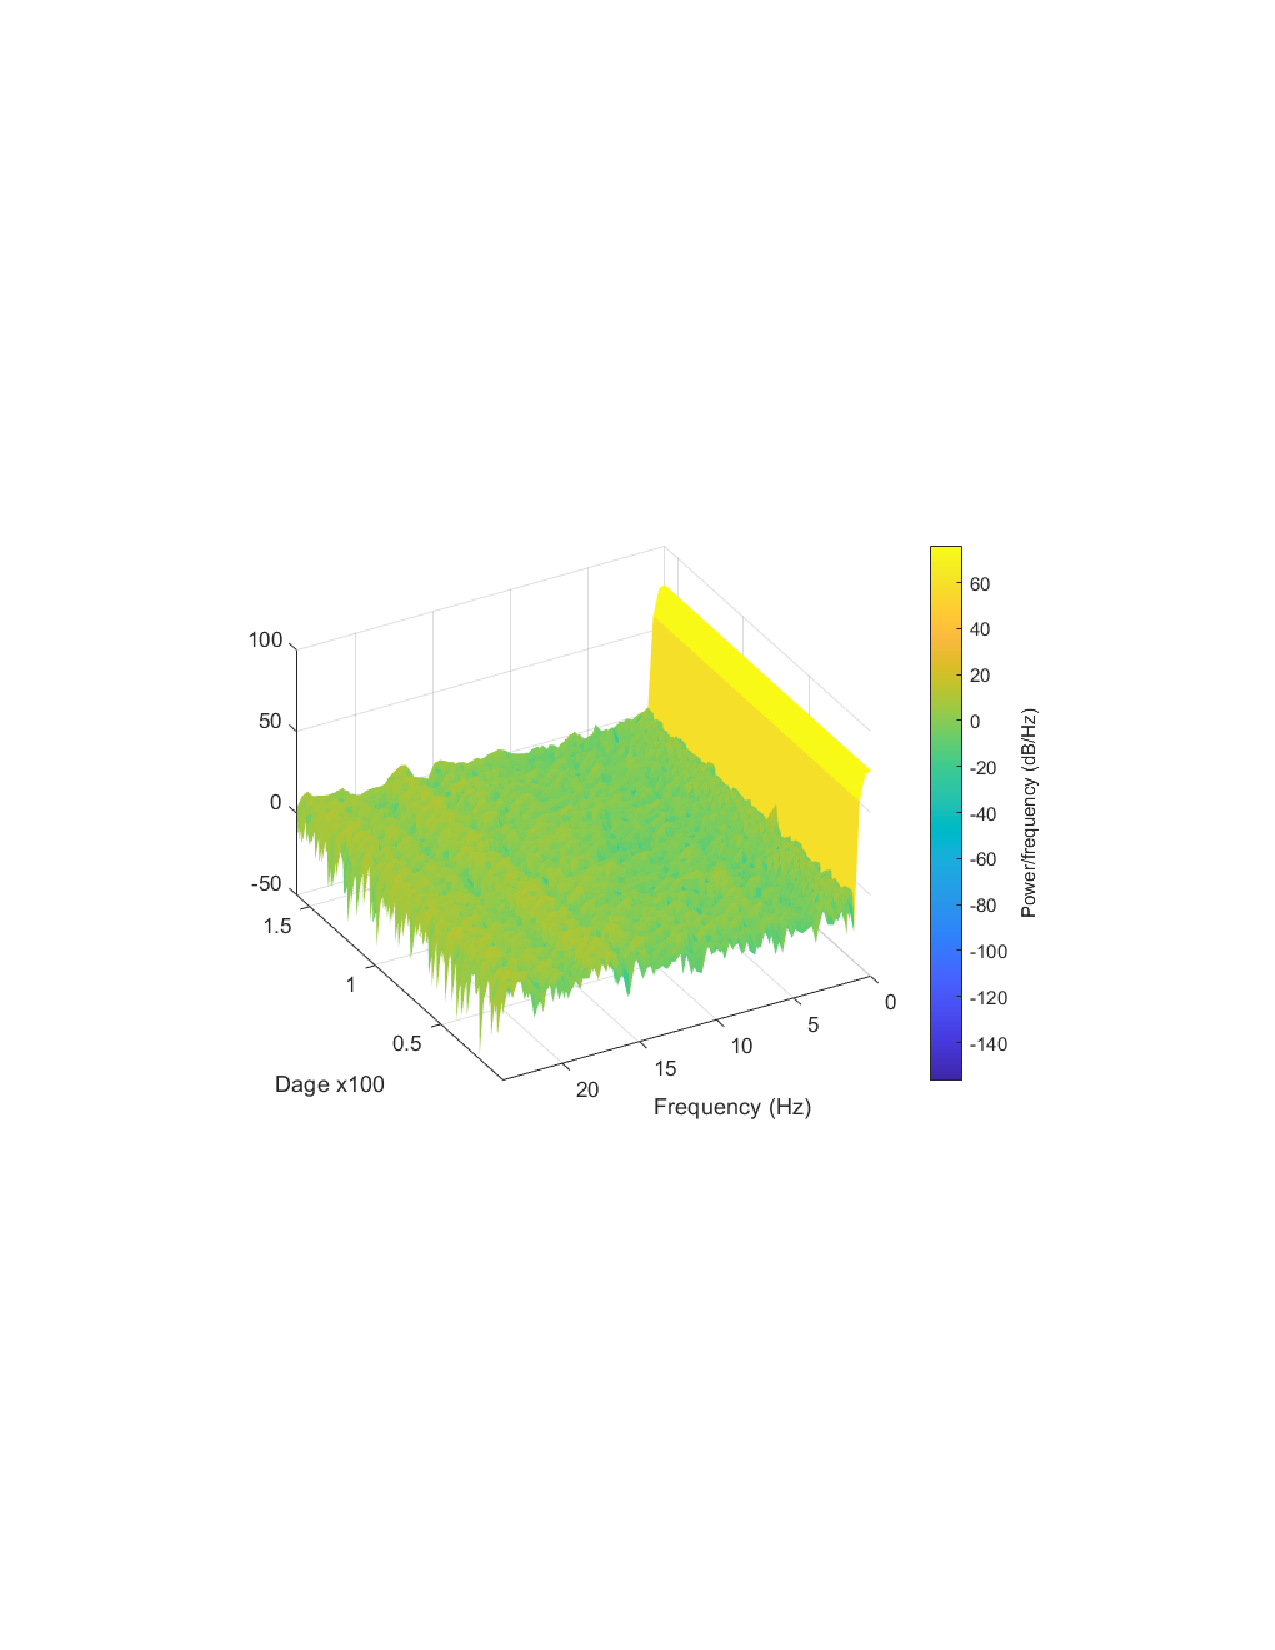
\includegraphics[width=\textwidth]{matlabstuff/mesh_stft.pdf}
  \caption{STFT spectrogram of the kepler data}%
  \label{fig:STFT}
\end{figure}

